\documentclass{ximera}
%% handout
%% space
%% newpage
%% numbers
%% nooutcomes

\usepackage{tikz}
\usepackage{tkz-euclide}
\usetkzobj{all}
\pgfplotsset{compat=1.7} % prevents compile error.

\tikzstyle geometryDiagrams=[ultra thick,color=blue!50!black]
 %% we can turn off input when making a master document

\outcome{Understand limits of functions}

\title{Limits of functions given graphically}

\begin{document}
\begin{abstract}
In this activity we will learn about limits of functions.
\end{abstract}
\maketitle

Consider the function whose graph is displayed below:
%\begin{image}
%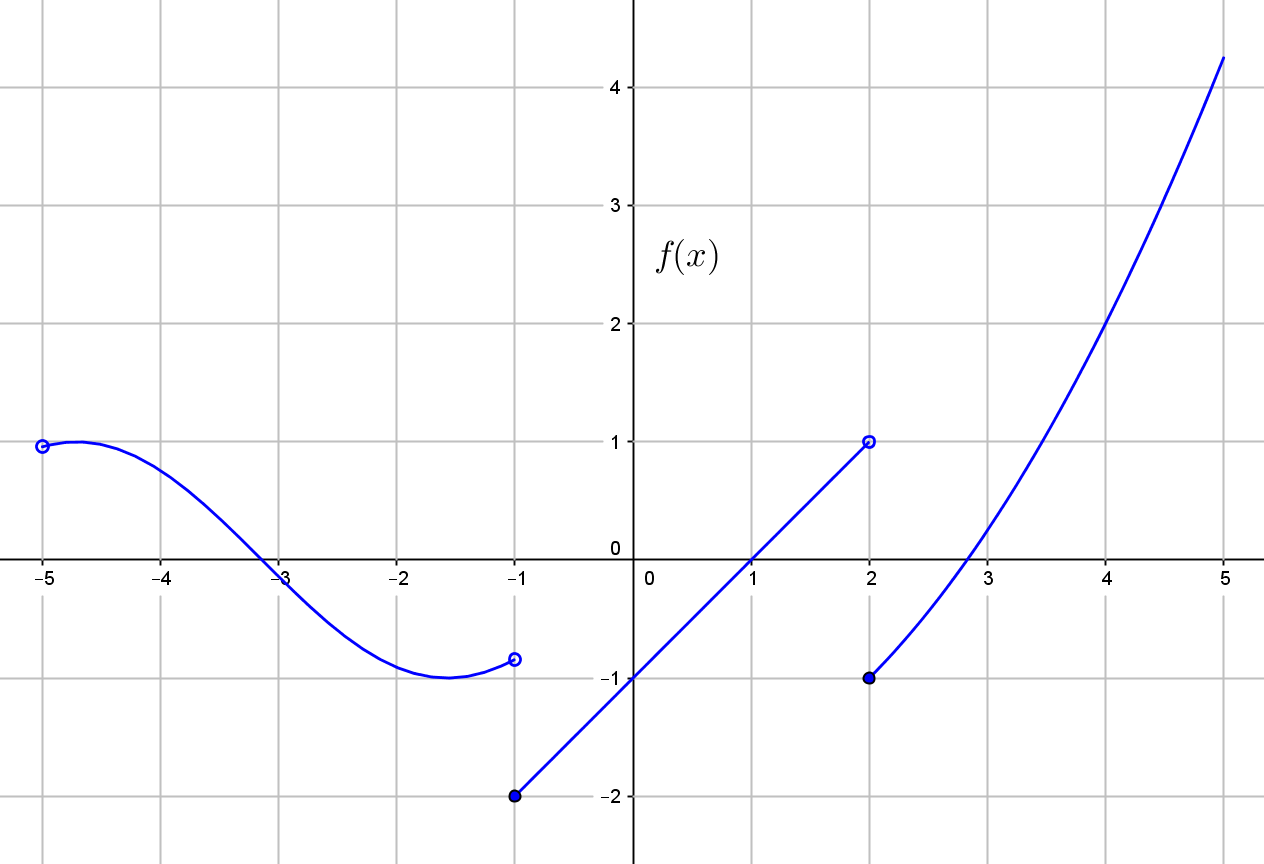
\includegraphics{pieceWise1.png}
%\end{image}

\begin{exercise}
Find 
\[
\lim_{x \to 1^+} f(x)=\answer{0}
\]
\end{exercise}

\begin{exercise}
Given that $r(v)=-2 v^2-4 v-4$, evaluate $r(-0.4)$. Express your answer in decimal notation.
\begin{hint}
$r(-0.4)=-2 (-0.4)^2-4 (-0.4)-4$.
\end{hint}
\begin{hint}
$r(-0.4)=-2.72$.
\end{hint}
The value of the function $r(v)=-2 v^2-4 v-4$, evaluated at $v=-0.4$, is $\answer{-2.72}$.
\end{exercise}

\begin{question}
What is the worst kind of cat?
\begin{prompt}
\begin{multipleChoice}
\choice{tabby}
\choice[correct]{puppy}
\choice{dog}
\choice{kitten}
\choice{main coon}
\end{multipleChoice}
\end{prompt}
\begin{hint}
It is not a cat or a type of cat.
\end{hint}
\begin{hint}
It is a puppy!
\end{hint}
\end{question}

\begin{exercise}
In the plot below, is $R$ a function of $n$?

\begin{image}
\begin{tikzpicture}
\begin{axis}[
            ymin=-5,
	    ymax=5,
            axis lines =center, xlabel=$n$, ylabel=$R$,
              every axis y label/.style={at=(current axis.above origin),anchor=south},
              every axis x label/.style={at=(current axis.right of origin),anchor=west},
            domain=-5:5,
            grid = major,
            xtick={-4,...,4},
            ytick={-4,...,4},
          ]
          \addplot [very thick, smooth] {4 + (-0.42857142857142855 + (-0.05952380952380952 + (0.09163059163059163 + (-0.041447441447441453 - 0.08955488955488956*(-3 + x))*(-2 + x))*(-0.5 + x))*(-3.5 + x))*(3.5 + x)};
        \end{axis}
\end{tikzpicture}
\end{image}
\end{exercise}


In the plot below, is $b$ a function of $w$?

\begin{image}
\begin{tikzpicture}
\begin{axis}[
            ymin=-5,
	    ymax=5,
            axis lines =center, xlabel=$w$, ylabel=$b$,
              every axis y label/.style={at=(current axis.above origin),anchor=south},
              every axis x label/.style={at=(current axis.right of origin),anchor=west},
            domain=-5:5,
            grid = major,
            xtick={-4,...,4},
            ytick={-4,...,4},
          ]
          \addplot [very thick, smooth] {2 + (3.5 + x)*(0.2857142857142857 + (-3.5 + x)*(0.489795918367347 + x*(0.34013605442176864 + (-0.5850340136054422 - 0.25117739403453676*(-0.5 + x))*(2 + x))))};
        \end{axis}
\end{tikzpicture}
\end{image}

Does not work
\end{document}
